% Experiments for Chapters 2 and 3 of the dissertation: setup, results and discussion.
% Protocol: dissertation/PROTOCOL.md. Data: ~/memprint-data/2026-11-05-diss-ch2.
% Tables and figures are generated, not typed:
%   PYTHONPATH=analysis ~/environments/memfp/bin/python -W ignore dissertation/score.py m1 plan m8 m4 m3 m6 m7 r1
%   PYTHONPATH=analysis ~/environments/memfp/bin/python -W ignore dissertation/figures.py
%   PYTHONPATH=analysis ~/environments/memfp/bin/python -W ignore dissertation/tables.py
\documentclass[11pt]{article}
\usepackage[margin=1in]{geometry}
\usepackage{booktabs}
\usepackage{array}
\usepackage{graphicx}
\usepackage{xcolor}
\usepackage[hidelinks]{hyperref}
\usepackage[font=small,labelfont=bf]{caption}
\graphicspath{{figures/}}
\newcommand{\tabinput}[1]{\input{tables/#1}}
\newcommand{\memprint}{MemPrint}

\title{Corrected Experiments for MemPrint (Chapter 2)\\and the Resident-Memory Model on MemPrint's Inputs (Chapter 3)}
\author{}
\date{November 6, 2026}

\begin{document}
\maketitle

\section{Overview}
\label{sec:overview}

This document reports the experiments that the dissertation plan lists for Chapters 2 and 3, together with the
corrections they make to the published \memprint{} results. The central change is the definition of the true
footprint. The published results count, for each start address, the largest access made from that address
(the \emph{start-address} truth). The chapter now uses the number of distinct bytes the program reads or writes
(the \emph{bytes-touched} truth), which is the definition that the motivation section and Chapter 3 use. Every
\memprint{} number in this document is computed under the bytes-touched truth, and every published number is
shown next to it as the original result.

The experiments answer five questions. First, whether the analysis pipeline reproduces the published accuracy,
and how much that accuracy changes under the bytes-touched truth (M1, M5 and M8). Second, whether the published
sampler labels its bins with the interval they actually sample (M2). Third, whether the sampler's bins behave
like the splitter's bins, on which every published test error was computed (M3). Fourth, how the heap profilers
compare with the corrected truth and how much the sampler costs (M6 and M7). Fifth, how the resident-memory model
of Chapter 3 performs on \memprint{}'s own inputs (R1). The protocol, including the decision rule of M3, was
committed before any run (commit \texttt{f32d036}), and Section~\ref{sec:amend} lists the two changes made after
the runs. The GPU experiments of Chapters 5 and 6 are out of scope here.

Table~\ref{tab:changes} summarizes the numbers in the chapter that change. Section~\ref{sec:setup} describes the
setup, Section~\ref{sec:ch2} the \memprint{} experiments, Section~\ref{sec:ch3} the resident-memory model, and
Section~\ref{sec:open} the questions that remain open.

\begin{table}[htbp]
\centering
\caption{Numbers in Chapter 2 that change. Published values are from the TACO paper and the chapter's tables;
corrected values are from this document. Errors are test MAPE in \%, at each subset's training-best interval,
over the 28 workloads (27 PolyBench kernels and miniVite).}
\label{tab:changes}
\small
\begin{tabular}{@{}>{\raggedright\arraybackslash}p{5.2cm}>{\raggedright\arraybackslash}p{4.4cm}>{\raggedright\arraybackslash}p{5.8cm}@{}}
\toprule
Quantity & Published & Corrected (source) \\
\midrule
L2O test MAPE, extrapolation & 9.78 & 11.88 (Table~\ref{tab:m1}) \\
L2O test MAPE, interpolation & 3.70 & 3.42 (Table~\ref{tab:m1}) \\
L2O maximum, extrapolation & 46.83 (atax) & 71.79 (bicg) \\
Largest test MAPE, any subset & 109.23 (trisolv, MT) & 99.56 (bicg, MT) \\
L2O on the sampler's own bins & not measured & 12.16 and 3.63 (Table~\ref{tab:m3}) \\
miniVite L2O, extrapolation and interpolation & 12.90 and 1.57 & 10.32 and 1.79 (Table~\ref{tab:m4mape}) \\
Bins per interval & 50 (text) & 20 (Section~\ref{sec:m8}) \\
Intervals used per workload & ``12 or 13'' & 9 to 13 (Table~\ref{tab:m8}) \\
Sampler wall time, miniVite 8,192 vertices & 42.1 s at 1 in 500; 52.2 s at 1 in 1,000; 46.1 s at 1 in 2,500
  & 30.9 s, 27.9 s and 25.6 s at those actual bin intervals (Table~\ref{tab:m7}) \\
Cumulative training cost & 216, 484 (438.77 in the text), 720 and 1,093 s & 46, 87 and 188 s
  (Figure~\ref{fig:cumulative}) \\
Heap profilers against the truth & ``substantially underestimate'' & gemm 0.12$\times$ to 0.92$\times$;
  miniVite 1.31$\times$ to 0.92$\times$ (Table~\ref{tab:m6}) \\
\bottomrule
\end{tabular}
\end{table}

\section{Setup}
\label{sec:setup}

\paragraph{Machine and software.}
All runs used one machine, the one on which the published overheads were measured. The machine has two Intel Xeon
E5-2620 v4 processors at 2.10 GHz (32 hardware threads) and 62 GiB of memory, and it runs Linux 4.18 with
glibc 2.28 and GCC 8.5.0. The tracing tools run on Pin 3.30. Every program ran with one OpenMP thread
(\texttt{OMP\_NUM\_THREADS=1}), which is the thread count of the bytes-touched retrace, and the runs ran one at a
time. The Pin tool used for all runs is a frozen copy of \texttt{pintool/memprint\_trace.cpp} at commit
\texttt{f32d036}.

\paragraph{Workloads and inputs.}
The workloads are the 27 PolyBench/C kernels of the published test table and miniVite. Each PolyBench kernel runs
at seven inputs (MINI, MINI2, MINI3, SMALL, SMALL2, SMALL3 and MEDIUM), four of which (MINI2, MINI3, SMALL2 and SMALL3) extend PolyBench's own datasets with intermediate sizes. miniVite runs on generated graphs of 1,024, 2,048, 4,096, 8,192 and 16,384
vertices. M5 adds durbin and jacobi-1d, which appear in the published tables but were not retraced before. As in
the published protocol, the extrapolation split (EXTRA) holds out each workload's largest input, and the
interpolation split (INTER) holds out the middle one when the inputs are ordered by true footprint.

\paragraph{Truth and model.}
The bytes-touched truth of an input is the number of distinct bytes that a complete trace of the run reads or
writes. The allocator's own references (glibc's chunk headers and free lists) count as time but not as footprint,
and the Pin tool gained a knob, \texttt{-exclude\_alloc}, that applies this rule without tracking frees. A bin's
observed footprint is the same quantity computed on one subsample of the references. \memprint{} predicts
$\alpha = \textit{truth} / \textit{observed}$ from a bin's observed footprint, its sampling interval and the
standard deviation of the observed footprint across the bins of the same interval, with a log-linear model of
seven terms. The three training subsets are NZ (every interval), MT (the intervals whose spread grows monotonically
with input size) and L2O (the best monotone interval with one interval below it and three above it). The analysis
is \texttt{analysis/memprint/build.py}, unchanged from the version that reproduces the published tables.

\paragraph{Splitter and samplers.}
The splitter assigns each reference to one of 20 disjoint bins at each of 13 intervals, from 1 in 100 to
1 in 100,000. The published sampler (\texttt{buffer\_memtrace\_poissonBS.cpp}) keeps 1 in $i$ references and
copies each kept reference into $K$ distinct bins out of $s$, where $K$ follows a Poisson distribution with mean
$\lambda = s/r$. The current tool implements the same bootstrap and, with \texttt{-disjoint 1}, a disjoint variant
in which each kept reference enters exactly one of $s$ bins, so that the bins are distributed as the splitter's
bins at interval $i \cdot s$ for the same instrumentation cost.

\section{Chapter 2: \memprint{}}
\label{sec:ch2}

\subsection{M1. The published protocol under the bytes-touched truth}
\label{sec:m1}

We ran the published protocol on three sets of tables: the published tables, the start-address retrace and the
bytes-touched retrace (with M4's miniVite). Table~\ref{tab:m1} gives the test MAPE of each subset at its
training-best interval, which is the basis of the published test table.

\begin{table}[htbp]
\centering
\caption{Test MAPE (\%) at each subset's training-best interval over the 28 workloads. ``Published tables''
reruns the unchanged pipeline on the published start-address tables. ``Bytes touched, splitter bins'' is the
corrected result. ``Sampler bins'' scores the same fitted models on the bootstrap sampler's own output at the
held-out input (M3, mean of 3 seeds).}
\label{tab:m1}
\small
\begin{tabular}{@{}llrrrrrrrr@{}}
\toprule
& & \multicolumn{3}{c}{Published tables} & \multicolumn{3}{c}{Bytes touched, splitter bins}
& \multicolumn{2}{c}{Sampler bins} \\
\cmidrule(lr){3-5}\cmidrule(lr){6-8}\cmidrule(l){9-10}
Split & Subset & Mean & Median & Max & Mean & Median & Max & Mean & Median \\
\midrule
\tabinput{m1}
\bottomrule
\end{tabular}
\end{table}

\paragraph{Reproduction.}
The pipeline reproduces the published results from the published tables to within 0.1 point. It gives an L2O test
MAPE of 9.72\% for extrapolation and 3.79\% for interpolation, against the published 9.78\% and 3.70\%, and it
reproduces the published maxima exactly (atax 46.83\% under L2O, trisolv 109.23\% under MT, and 2mm 21.62\% under
MT for interpolation). The start-address retrace gives tables identical to the published ones, so the retrace
changes nothing except the truth definition. The residual of 0.06 and 0.09 points remains unexplained. Rounding the
coefficients to four decimals, as the published scripts did, does not explain it, because rounding moves the
extrapolation error to 10.12\% (away from 9.78\%) and the interpolation error to 3.75\%.

\paragraph{Corrected accuracy.}
Under the bytes-touched truth, the L2O test MAPE is 11.88\% for extrapolation and 3.42\% for interpolation. The
extrapolation error grows by 2.1 points on average, while its median falls from 6.90\% to 6.09\%, so the increase
comes from a few workloads with large errors. Per workload (Table~\ref{tab:l2o}), 16 of the 28 workloads extrapolate
worse and 12 better, and 12 interpolate worse and 16 better. The largest changes are bicg (21.71\% to 71.79\%),
trmm (2.20\% to 29.51\%), trisolv (7.76\% to 26.57\%) and seidel-2d (9.44\% to 26.40\%) for the worse, and
cholesky (38.14\% to 3.10\%), atax (46.83\% to 20.24\%) and adi (20.43\% to 5.16\%) for the better.

The truth itself barely changes for PolyBench. A PolyBench kernel's bytes-touched truth is 470 to 1,400 bytes
below its start-address truth, under 1.2\% at every input, because the kernels access aligned arrays with accesses
of one size. What changes is the observed footprint of each bin, which under the start-address definition counts
the largest access from each start address that the bin happens to contain. At 1 in 1,000, gemm's mean bin
footprint at MEDIUM falls from 317,110 to 288,335 bytes (9.1\%), so $\alpha$ and the fitted coefficients move
even though the truth does not. The new errors therefore reflect a different relation between bins and truth, and
the tail of large errors (bicg, trmm, trisolv and seidel-2d) comes from kernels whose training-best interval is
sparse (1 in 5,000 to 1 in 10,000), which is consistent with the few references that a bin holds at those
intervals. For miniVite the truth does change, and the
bytes-touched truth is 25\% to 39\% below the start-address truth (Section~\ref{sec:m4}).

\begin{table}[htbp]
\centering
\caption{L2O test MAPE (\%) per workload at the training-best interval $k$ (1 in $k$). ``Published'' reruns the
pipeline on the published tables. ``Bytes'' is the corrected result on splitter bins, and ``Sampler'' scores the
same model on the bootstrap sampler's bins at the held-out input (mean of 3 seeds).}
\label{tab:l2o}
\small
\begin{tabular}{@{}lrrrrrrrr@{}}
\toprule
& \multicolumn{4}{c}{Extrapolation (largest input)} & \multicolumn{4}{c}{Interpolation (middle input)} \\
\cmidrule(lr){2-5}\cmidrule(l){6-9}
Workload & Published & Bytes & $k$ & Sampler & Published & Bytes & $k$ & Sampler \\
\midrule
\tabinput{l2o}
\bottomrule
\end{tabular}
\end{table}

Two differences between the sets of tables affect individual rows. First, heat-3d has seven inputs in the retrace
and five in the published table, so its interpolation input is SMALL in the retrace and SMALL2 in the published
table. Second, the intervals that a workload drops differ between the sets (Section~\ref{sec:m8}).

Figure~\ref{fig:sd} redraws the chapter's figure of the spread across bins for gemm under the bytes-touched
truth. Five intervals remain monotone (1 in 250, 500, 750, 5,000 and 10,000), and the figure supports the same
argument as before. At a fixed interval the spread grows with the input, so it carries information about the
input's size that the observed footprint alone does not.

\begin{figure}[htbp]
\centering
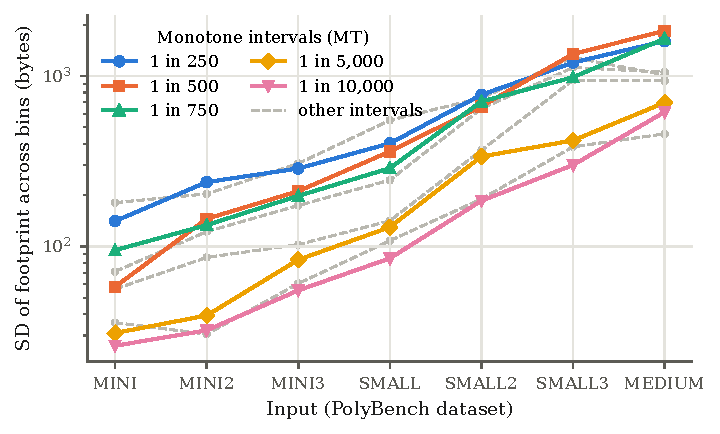
\includegraphics[width=0.7\linewidth]{sd_gemm}
\caption{Standard deviation of the observed footprint across the 20 splitter bins against the input, gemm, under
the bytes-touched truth. Solid lines are the intervals whose spread grows monotonically with the input (the MT
subset), and dashed gray lines are the other intervals up to 1 in 10,000. The vertical axis is logarithmic.}
\label{fig:sd}
\end{figure}

\subsection{M2. What the published sampler's bins actually sample}
\label{sec:m2}

The published sampler names its bins \texttt{SubSample\_}$\langle i \cdot s / r\rangle$, that is, $i\lambda$. A
bin's inclusion probability for a kept reference is $E[\min(K, s)]/s \approx \lambda/s = 1/r$, so a bin samples
about 1 in $i \cdot r$ references. The label equals the interval only when $s = r^2$, which holds for the defaults
$s=100$ and $r=10$. The chapter's worked example ($i = 1{,}000$, 50 bins and $r = 20$) would be labelled
1 in 2,500 while each bin samples about 1 in 20,000. The sampler also stores addresses as 32-bit integers, which
truncates them, and it does not cap $K$ at $s$.

We measured every sampler run on disk. For each run, the empirical bin interval is $i$ times the run's kept
references divided by the bin's reference count. Table~\ref{tab:m2} gives the ratio of the label to the empirical
interval for each set of runs.

\begin{table}[htbp]
\centering
\caption{The bin label against the bin's measured interval, for every set of sampler runs on disk. A ratio of 1
means the label is right. The first row is the published sampler, and the other rows are older tools whose runs feed
no published number.}
\label{tab:m2}
\small
\begin{tabular}{@{}lrlrrr@{}}
\toprule
& & & \multicolumn{3}{c}{Label / measured interval} \\
\cmidrule(l){4-6}
Run set & Runs & Bins & Min & Median & Max \\
\midrule
\tabinput{m2}
\bottomrule
\end{tabular}
\end{table}

No published accuracy number used a mislabelled bin. Every table behind the published predictions is splitter
output, whose labels are exact, and the published test MAPE is computed on the splitter's bins at the held-out
input rather than on any sampler's output. The published overheads, however, did use mislabelled runs. They come
from the published sampler with $s=50$ and $r=5$, whose bins are labelled $i \cdot 10$ and sample 1 in $i \cdot 5$,
and the plotting script draws them at the label. The chapter's ``42.1 s at 1 in 500'' is the run with $i = 50$,
whose bins sample about 1 in 250 and whose instrumentation keeps 1 in 50 references. The values 52.2 s and 46.1 s
that the text gives for 1 in 1,000 and 1 in 2,500 do not appear in any log. Section~\ref{sec:m7} replaces all three.

\subsection{M3. Do the sampler's bins behave like the splitter's?}
\label{sec:m3}

Because the published test error is computed on splitter bins, it assumes that a sampler's bins are distributed
like the splitter's. Under the bootstrap a replicated reference enters several bins, so the bins are positively
correlated, and we expected the spread across them, which is a model feature, to be smaller than across the
splitter's disjoint bins. To test this, we ran both samplers at every interval that a fitted model uses for
prediction, at the extrapolation and interpolation inputs of all 28 workloads, with 3 seeds each (972 runs). The
bootstrap used the published defaults ($s=100$, $r=10$, $i=k/10$), and the disjoint sampler used 20 bins
($i=k/20$), so both sample about 1 in $k$ per bin. We then scored each workload's fitted models on the sampler's
bins.

\begin{table}[htbp]
\centering
\caption{Sampler bins against splitter bins at the same interval and input (M3, 972 runs). The ratios compare
each run's bins with the 20 splitter bins at the same interval. ``MAPE difference'' is the median over workloads,
splits and subsets of the sampler-bin MAPE minus the splitter-bin MAPE, in points. The last two columns are the
mean L2O MAPE (\%) on the sampler's bins.}
\label{tab:m3}
\footnotesize
\setlength{\tabcolsep}{4pt}
\begin{tabular}{@{}lrrcrrr@{}}
\toprule
& \multicolumn{3}{c}{Ratio to splitter bins} & & \multicolumn{2}{c}{L2O MAPE (\%)} \\
\cmidrule(lr){2-4}\cmidrule(l){6-7}
Sampler & Mean, med. & SD, med. & SD, 10th to 90th pct. & MAPE diff. & EXTRA & INTER \\
\midrule
\tabinput{m3}
\bottomrule
\end{tabular}
\end{table}

\begin{figure}[htbp]
\centering
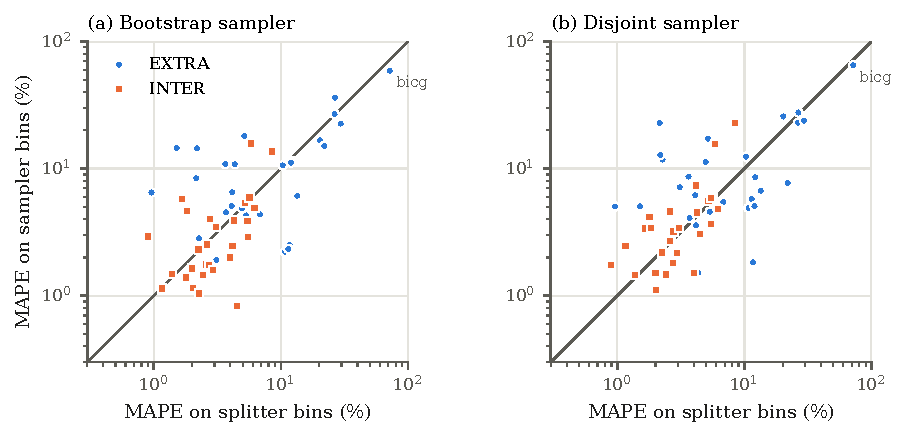
\includegraphics[width=\linewidth]{m3}
\caption{L2O test MAPE per workload on the sampler's bins (mean of 3 seeds) against on the splitter's bins, at the
training-best interval. Points on the diagonal have the same error. Both axes are logarithmic.}
\label{fig:m3}
\end{figure}

The bootstrap's bins are close to the splitter's (Table~\ref{tab:m3} and Figure~\ref{fig:m3}). Their mean
footprint is 0.998 of the splitter's at the median, and their spread is 0.938 of the splitter's, which is smaller
as expected but by only 6\%. Across workloads the sampler-bin MAPE is 0.16 point above the splitter-bin MAPE at
the median. Under the decision rule fixed before the runs, the chapter reports the bootstrap, because the MAPE
difference is below 2 points and the median spread ratio lies between 0.9 and 1.1. With the sampler's own bins,
the L2O error is 12.16\% for extrapolation and 3.63\% for interpolation, 0.28 and 0.21 point above the splitter
bins. The disjoint sampler is not more accurate (12.32\% and 4.42\%), although its median spread ratio of 0.964 is
closer to 1, so the bootstrap's correlation between bins has no measurable cost here.

The per-workload spread is wider than the averages suggest. Between the 10th and 90th percentiles of runs, the
spread ratio ranges from 0.72 to 1.18 for the bootstrap, and individual workloads move by several points in both
directions in Figure~\ref{fig:m3}, for example 3mm (4.34\% to 10.84\% for extrapolation) and 2mm (11.71\% to
2.51\%). Three seeds per run therefore matter for a per-workload claim, while the aggregate changes little.

\subsection{M4. miniVite under the bytes-touched truth}
\label{sec:m4}

We retraced miniVite at all five inputs with the splitter under the bytes-touched truth and with the allocator's
references excluded. Table~\ref{tab:m4truth} compares the three truths. The bytes-touched truth is 25\% to 39\%
below the start-address truth, and the gap shrinks as the graph grows. miniVite makes many overlapping accesses
of different sizes to the same objects, and the start-address definition counts the largest access from each
start address in full, so overlapping accesses are counted more than once. Excluding the allocator's own
references lowers the truth by a further 1.0\% to 2.6\%, about 111,000 bytes at every input.

\begin{table}[htbp]
\centering
\caption{miniVite's true footprint (bytes) under three definitions, and the change of the corrected truth (\%)
against the other two.}
\label{tab:m4truth}
\small
\begin{tabular}{@{}rrrrrr@{}}
\toprule
Vertices & Start address & Bytes, with allocator & Bytes touched & vs.\ with allocator & vs.\ start address \\
\midrule
\tabinput{m4_truth}
\bottomrule
\end{tabular}
\end{table}

\begin{table}[htbp]
\centering
\caption{miniVite's test MAPE (\%) at the training-best interval $k$, against the published values.}
\label{tab:m4mape}
\small
\begin{tabular}{@{}llrrrr@{}}
\toprule
Split & Subset & Published & $k$ & Bytes, splitter bins & Bytes, sampler bins \\
\midrule
\tabinput{m4_mape}
\bottomrule
\end{tabular}
\end{table}

Under the corrected truth, miniVite's L2O error is 10.32\% for extrapolation and 1.79\% for interpolation, against
the published 12.90\% and 1.57\% (Table~\ref{tab:m4mape}). The chapter's claim that MT is consistently best for
miniVite no longer holds. MT extrapolates worst (15.72\%), NZ best (3.17\%), and on the sampler's own bins L2O and
NZ are within 0.5 point of each other. Figure~\ref{fig:alpha} redraws the chapter's two figures of $\alpha$ for
miniVite. As before, $\alpha$ falls with the input at every interval and rises in proportion to the interval at
every input, which is the structure the model's terms capture.

\begin{figure}[htbp]
\centering
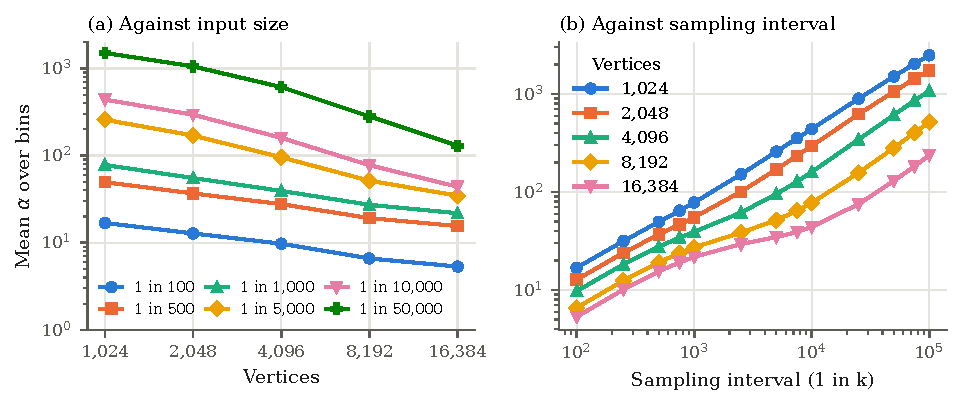
\includegraphics[width=\linewidth]{alpha_minivite}
\caption{miniVite, mean $\alpha$ (bytes-touched truth over a bin's observed footprint) over the 20 splitter bins:
(a) against the input at six intervals and (b) against the interval at each input. Both vertical axes and the
horizontal axis of (b) are logarithmic.}
\label{fig:alpha}
\end{figure}

\paragraph{Training cost against accuracy.}
Figure~\ref{fig:cumulative} redraws the chapter's figure of accuracy against training cost. Each point trains on
the inputs up to $n$ vertices and tests on 16,384 vertices, with the MT and L2O subsets chosen from the training
inputs alone. The cost is the splitter's wall time summed over the training inputs, measured in M4. The published
figure starts at 1,024 vertices, but a single training input yields no monotone interval and too few points to fit
seven terms reliably, so the redrawn figure starts at 2,048. Adding inputs improves every subset. With all four
training inputs, NZ reaches 3.17\%, L2O 10.32\% and MT 15.72\%, for 188 s of splitter time. The published
cumulative costs (216, 484, 720 and 1,093 s) are hardcoded in the plotting script and are not reproduced by any
run. The chapter's 438.77 s is a transposition of the script's 483.77 s.

\begin{figure}[htbp]
\centering
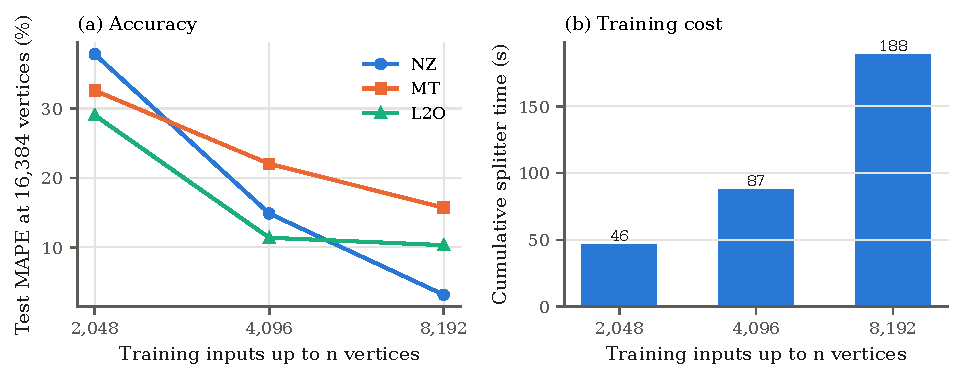
\includegraphics[width=\linewidth]{cumulative}
\caption{miniVite: (a) test MAPE at 16,384 vertices when training on the inputs up to $n$ vertices, and (b) the
splitter's cumulative wall time over those training inputs.}
\label{fig:cumulative}
\end{figure}

\subsection{M5. The two kernels missing from the retrace}
\label{sec:m5}

durbin and jacobi-1d traced without error at all seven inputs. Neither has a monotone interval, so only the NZ
subset can be fitted, as in the published tables, where jacobi-1d appears in training only and durbin not at all.
Their NZ test MAPE is 1.07\% and 0.36\% for durbin and 1.06\% and 0.19\% for jacobi-1d (extrapolation and
interpolation). The chapter's MT and L2O averages therefore remain over 28 workloads, and its NZ table can list 30.

\subsection{M6. Heap profilers against the corrected truth}
\label{sec:m6}

We ran Massif and DHAT on gemm at its seven inputs and miniVite at its five, the workloads of the chapter's
Figure 1. Table~\ref{tab:m6} and Figure~\ref{fig:valgrind} compare their peaks with the bytes-touched truth, and
with \memprint{}'s L2O estimate from the bootstrap sampler at the extrapolation and interpolation inputs. Massif
and DHAT agree with each other to within 5\% at every input, because both report the peak of live heap bytes.

\begin{table}[htbp]
\centering
\caption{Peak heap reported by Massif and DHAT against the bytes-touched truth (bytes), and the ratio of each
estimate to the truth. \memprint{} is the L2O estimate from the bootstrap sampler at the held-out input (mean of
3 seeds).}
\label{tab:m6}
\small
\begin{tabular}{@{}llrrrrrl@{}}
\toprule
& & & & & \multicolumn{3}{c}{Estimate / truth} \\
\cmidrule(l){6-8}
Workload & Input & Truth & Massif & DHAT & Massif & DHAT & \memprint{} \\
\midrule
\tabinput{m6}
\bottomrule
\end{tabular}
\end{table}

\begin{figure}[htbp]
\centering
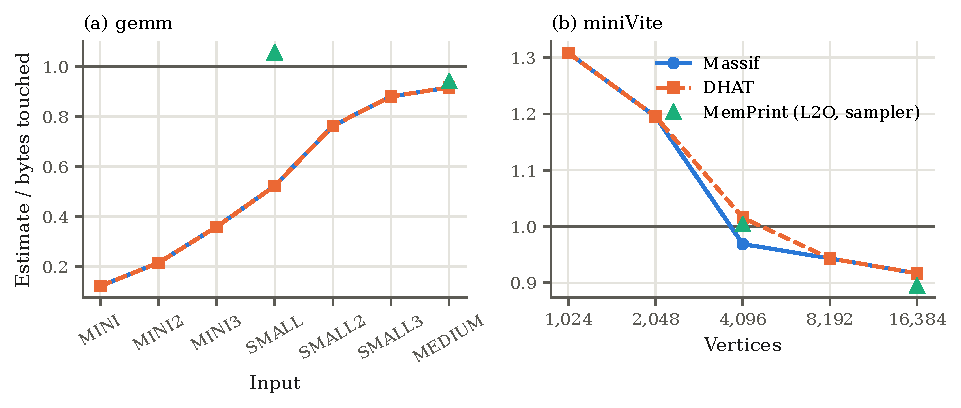
\includegraphics[width=\linewidth]{valgrind}
\caption{Estimate over the bytes-touched truth for Massif, DHAT and \memprint{} (L2O, bootstrap sampler, at the
held-out inputs only): (a) gemm and (b) miniVite. The horizontal line marks an exact estimate.}
\label{fig:valgrind}
\end{figure}

The direction of the heap profilers' error depends on the workload and the input. For gemm they underestimate at
every input, from 0.12$\times$ at MINI to 0.92$\times$ at MEDIUM. The truth counts every byte the process touches,
including its stack, static data and the C runtime's share, about 107,000 bytes for these kernels, while the heap
profilers count only the heap, so the gap dominates at the small inputs and shrinks as the arrays grow. For
miniVite the heap profilers overestimate at the two smallest inputs (1.31$\times$ and 1.20$\times$), where
miniVite allocates memory that it never touches, and underestimate from 8,192 vertices on (0.94$\times$ and
0.92$\times$), where the non-heap memory of the run outweighs the untouched heap. The paper on scheduling measured
1.42$\times$ to 1.55$\times$ for miniVite at 32,768 and 65,536 vertices, sizes outside this range, so the two
results do not conflict but show that the error changes sign with the input.

The chapter's statement that Massif and DHAT ``substantially underestimate'' is therefore true for gemm and for
the largest miniVite inputs, and false for the smallest miniVite inputs. \memprint{}'s estimate is within 7\% of
the truth at three of the four held-out inputs (0.94$\times$ and 1.05$\times$ for gemm, 1.00$\times$ for miniVite
at 4,096 vertices) and 0.89$\times$ at 16,384 vertices. At the largest inputs it is no closer than the heap
profilers, which are within 9\% there, but unlike them it does not depend on the input's mix of heap and non-heap
memory.

\subsection{M7. What the sampler costs}
\label{sec:m7}

We timed each sampler on miniVite at 8,192 vertices, as the chapter does, with 5 interleaved rounds and nothing
else running. Because M2 showed that the published labels are not the bin intervals, we timed each sampler at
matched bin intervals of 1 in 500, 1,000 and 2,500. For the published sampler we used both the published setting
($s=50$, $r=5$, $i=k/5$) and the defaults ($s=100$, $r=10$, $i=k/10$). The protocol's original timing at
$i = 500$, 1,000 and 2,500 with $s=50$ and $r=20$ was also run. Its bins sample 1 in 10,000 to 1 in 50,000, so we do
not report it.

\begin{table}[htbp]
\centering
\caption{Wall time (s) on miniVite at 8,192 vertices at matched bin intervals, median of 5 rounds, with the
slowdown over the native run (0.21 s) in parentheses. Instrumentation only runs the tool with sampling off.}
\label{tab:m7}
\small
\begin{tabular}{@{}lrrr@{}}
\toprule
Sampler & 1 in 500 & 1 in 1,000 & 1 in 2,500 \\
\midrule
\tabinput{m7}
\bottomrule
\end{tabular}
\end{table}

\begin{figure}[htbp]
\centering
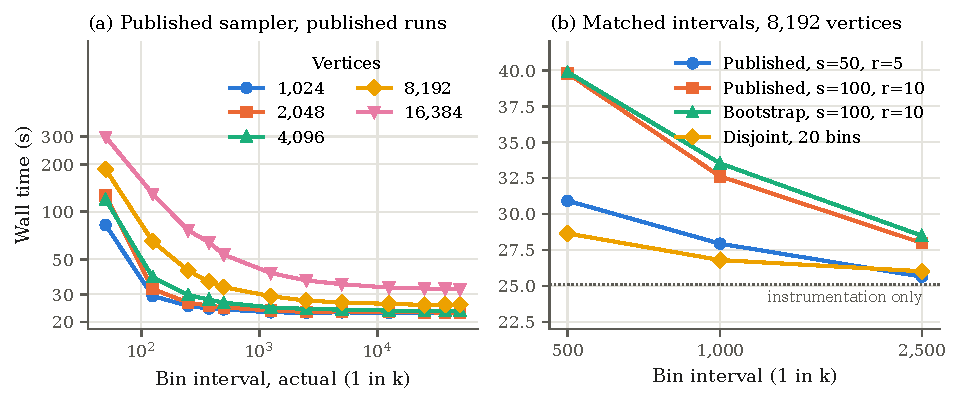
\includegraphics[width=\linewidth]{overhead}
\caption{Sampler wall time on miniVite. (a) The published runs of the published sampler ($s=50$, $r=5$), redrawn
at the bins' actual interval $5i$ instead of the label $10i$, with both axes logarithmic. (b) Each sampler at
matched bin intervals at 8,192 vertices, median of 5 rounds. The dotted line is the tool with sampling off.}
\label{fig:overhead}
\end{figure}

Table~\ref{tab:m7} and Figure~\ref{fig:overhead} give the corrected overheads. At the published setting, the
published sampler takes 30.9 s at 1 in 500, 27.9 s at 1 in 1,000 and 25.6 s at 1 in 2,500, against the 42.1 s,
52.2 s and 46.1 s of the chapter. The published log has 33.3 s for the run that sampled 1 in 500 on this machine,
8\% above the new measurement, so the machine measures as before and the difference from the chapter comes from the
labels. Most of the cost is Pin's instrumentation. Running the tool with sampling off already takes 25.1 s, a
115$\times$ slowdown, and sampling adds 0.5 to 15 s on top of it, depending on how many references a setting keeps.
The current tool's bootstrap costs the same as the published sampler at the same setting (39.9 s against 39.8 s
at 1 in 500). The disjoint sampler is the cheapest at every interval (28.7 s at 1 in 500, 28\% below the
bootstrap), because it copies each kept reference into one bin rather than about ten. The splitter, which records
all 13 intervals at once and is the cost of training, takes 87.7 s.

\subsection{M8. Bins, intervals and the training overhead}
\label{sec:m8}

Every table, published and retraced, has 20 bins per interval at every input, not the 50 that the chapter's text
states, and 13 intervals from 1 in 100 to 1 in 100,000, with no interval of 1 in 10. The pipeline drops an interval
for a workload when one of its bins observes no reference at some input, which happens at the sparsest intervals
of the smallest inputs. Table~\ref{tab:m8} lists the workloads that drop intervals. Under the bytes-touched truth,
14 of the 28 workloads use fewer than 13 intervals, against 11 in the published tables, and trisolv uses only 9, so the chapter's ``12 or 13
intervals'' should read ``9 to 13''.

\begin{table}[htbp]
\centering
\caption{Workloads that drop intervals, with the number of intervals used and the intervals dropped (1 in $k$) in the
published tables and in the bytes-touched retrace. The other 13 workloads use all 13 intervals in both.}
\label{tab:m8}
\small
\begin{tabular}{@{}lrlrl@{}}
\toprule
& \multicolumn{2}{c}{Published tables} & \multicolumn{2}{c}{Bytes touched} \\
\cmidrule(lr){2-3}\cmidrule(l){4-5}
Workload & Used & Dropped & Used & Dropped \\
\midrule
\tabinput{m8}
\bottomrule
\end{tabular}
\end{table}

\section{Chapter 3: the resident-memory model on \memprint{}'s inputs}
\label{sec:ch3}

\subsection{R1. Setup}
We ran each of the 27 PolyBench kernels at its seven inputs and miniVite at its five natively, 3 times each, under
the shim that samples \texttt{/proc/self/smaps\_rollup} every 1 ms, which Chapter 3 found to be the best sampler for
short runs. The truth is the bytes-touched truth of the same input. Both quantities cover the whole run, and the
PolyBench kernels allocate their arrays once, so the peak of memory in use should equal the bytes touched up to the
runtime's share.

We scored three predictions of the footprint, as in Chapter 3's blind test. Prediction (a) is the largest
anonymous memory minus the allocator's free memory during the run, the median of 3 runs. Prediction (b) adds to
(a) a constant $R$, the median of truth minus (a) over the other workloads' inputs, which is about 153,000 bytes.
Prediction (c) is Chapter 3's transfer rule, a linear fit of (a) against the input size over the workload's other
inputs, evaluated at the held-out input, plus $R$. The input size is the number of array elements the kernel
declares at that dataset, from its header, and the number of vertices for miniVite.

\subsection{R1. Results}

\begin{table}[htbp]
\centering
\caption{The resident-memory model at the held-out inputs of the 28 workloads. The model's columns give the absolute error against the
bytes-touched truth (\%) as mean / median, next to \memprint{}'s L2O test MAPE (\%), mean / median. The last column
counts the workloads within 10\% for (b) and (c).}
\label{tab:r1}
\footnotesize
\setlength{\tabcolsep}{4pt}
\begin{tabular}{@{}lrrrrrr@{}}
\toprule
& \multicolumn{3}{c}{Resident-memory model} & \multicolumn{2}{c}{\memprint{} L2O} & \\
\cmidrule(lr){2-4}\cmidrule(lr){5-6}
Split & (a) Measured & (b) Measured $+R$ & (c) Transfer $+R$ & Splitter bins & Sampler bins & Within 10\% \\
\midrule
\tabinput{r1}
\bottomrule
\end{tabular}
\end{table}

At the largest inputs, measuring the run natively and adding the constant $R$ is more accurate than \memprint{}
(Table~\ref{tab:r1}). Prediction (b) has a median error of 2.82\% and a mean of 5.90\%, with 26 of 28 workloads
within 10\%, against \memprint{}'s 9.49\% median and 12.16\% mean on the sampler's bins. Prediction (b) costs one
native run, a fraction of a second here, against one sampled Pin run of 25 s or more. The two exceptions are
trisolv, which (b) overestimates by 80\% because its measured peak at MEDIUM (1.21 MB) exceeds the truth
(0.75 MB), and trmm, overestimated by 18\%.

At the middle inputs, the native measurement fails. Prediction (b) has a median error of 24.36\% and only 2 of 28
workloads within 10\%. At SMALL, a PolyBench kernel runs for a few milliseconds and its arrays occupy about 100 kilobytes or less, so a 1 ms sampler often reads the process before the arrays are touched, and 6 of the 28 runs measure no
memory above the free memory at all. The transfer rule (c), which predicts the middle input from the other inputs,
recovers much of the accuracy, with a median of 4.97\% and 21 of 28 within 10\%, but \memprint{} is still better
there (2.49\% median on the sampler's bins). At the largest inputs the transfer rule is worse than measuring
directly (8.97\% median and an 88.8\% maximum for mvt), because the small inputs it extrapolates from are the ones
the sampler measures poorly. The interpolation column of (c) uses the floor of Chapter 3's post hoc variant (the
largest peak of the smaller inputs only), and the protocol fixed only the extrapolation column.

The comparison therefore splits by run length rather than by method. For a run long enough for the sampler to see
its peak, a native measurement plus a constant is cheaper and more accurate than \memprint{}. For runs of a few
milliseconds, \memprint{}'s trace sees every reference and the native sampler does not, and Chapter 3's own
limitation on short runs applies.

\section{Changes to the protocol after the runs}
\label{sec:amend}

Two changes were made after the runs and are marked in \texttt{dissertation/PROTOCOL.md}. First, the protocol's
timing (M7) ran at $i = 500$, 1,000 and 2,500, as the plan states. M2 then showed that the published numbers were
measured at different bin intervals, so we added the matched-interval timing of Section~\ref{sec:m7} and report it
instead. Second, R1's transfer rule needs each input's size, which the protocol did not define. We used the number
of declared array elements. The decision rule of M3 and every other analysis ran as written.

\section{Open questions}
\label{sec:open}

The reproduction of M1 leaves a residual of 0.06 and 0.09 point that rounding does not explain. Comparing the
published per-workload coefficients with the refitted ones would locate it, but no published number depends on it.
The chapter's 52.2 s and 46.1 s cannot be traced to any log, so the chapter should replace them rather than explain
them. The heap-profiler comparison covers gemm and miniVite only, and the sign change for miniVite rests on five
inputs and one run each. Finally, R1 shows that the resident-memory model needs runs longer than its sampling
period, and Chapter 3 should state this limit with the PolyBench numbers above.

\end{document}
